\documentclass{beamer}
\usepackage{amsmath}
\usepackage{amssymb}
\usepackage{physics}
\usepackage{amsthm}
\usepackage{graphicx}
\usepackage{caption}
\usepackage{subcaption}
\usepackage{listings}
\graphicspath{ {./figures/} }
\title{Aplikace spektrální metody}
\author{Dominika Hájková, Matyáš Fuksa, Ondřej Kureš}
\institute{Stormtrooperz}
\date{2021}

\begin{document}


\frame{\titlepage}
\begin{frame}
\frametitle{Spektrální metoda - Co to je?}
Povíme něco o spektrální metodě jako takové.
\end{frame}

\begin{frame}[fragile]
\frametitle{Trám na jiný způsob - kód}
\begin{lstlisting}[language=Matlab, basicstyle=\small, numbers=left,breaklines=true]
f = @(x) 75*9.81*exp(-x.^2/(2*0.01)); alpha = 0; beta = 0; gama = 0 ;delta = 0; n = 18; E = 9.4*10^6; Izz = 3;l = 10;X = [-l/2,l/2];
L = E*Izz*diffmat([n n+4],4,X);
vT = diffrow(n+4,0,-l/2,X); wT = diffrow(n+4,0,l/2,X); uT = diffrow(n+4,1,-l/2,X); sT = diffrow(n+4,1,l/2,X);
A = [L; vT; wT; uT; sT];
rhs = [gridsample(f,n); alpha; beta; gama; delta];
u = A\rhs;
tiledlayout(2,1)
nexttile
plot(chebfun(-u,X),'.-');ylim([-1 1]);
nexttile
plot(chebfun(-u,X),'.-');ylim([-0.001 0.001])
\end{lstlisting}
\end{frame}

\begin{frame}
\frametitle{Trám na jiný způsob - obrázky}
\centering
\begin{figure}
\includegraphics[width=.9\linewidth]{První.png}
\includegraphics[width=.9\linewidth]{Druhý.png}
\caption{Musím doplnit}
\end{figure}
\end{frame}

\begin{frame}
\frametitle{Kmitání membrán - Jak vypadá obdélník?}
\end{frame}


\begin{frame}
\begin{center}
\begin{huge}
Děkujeme za pozornost
\end{huge}
  \centering
  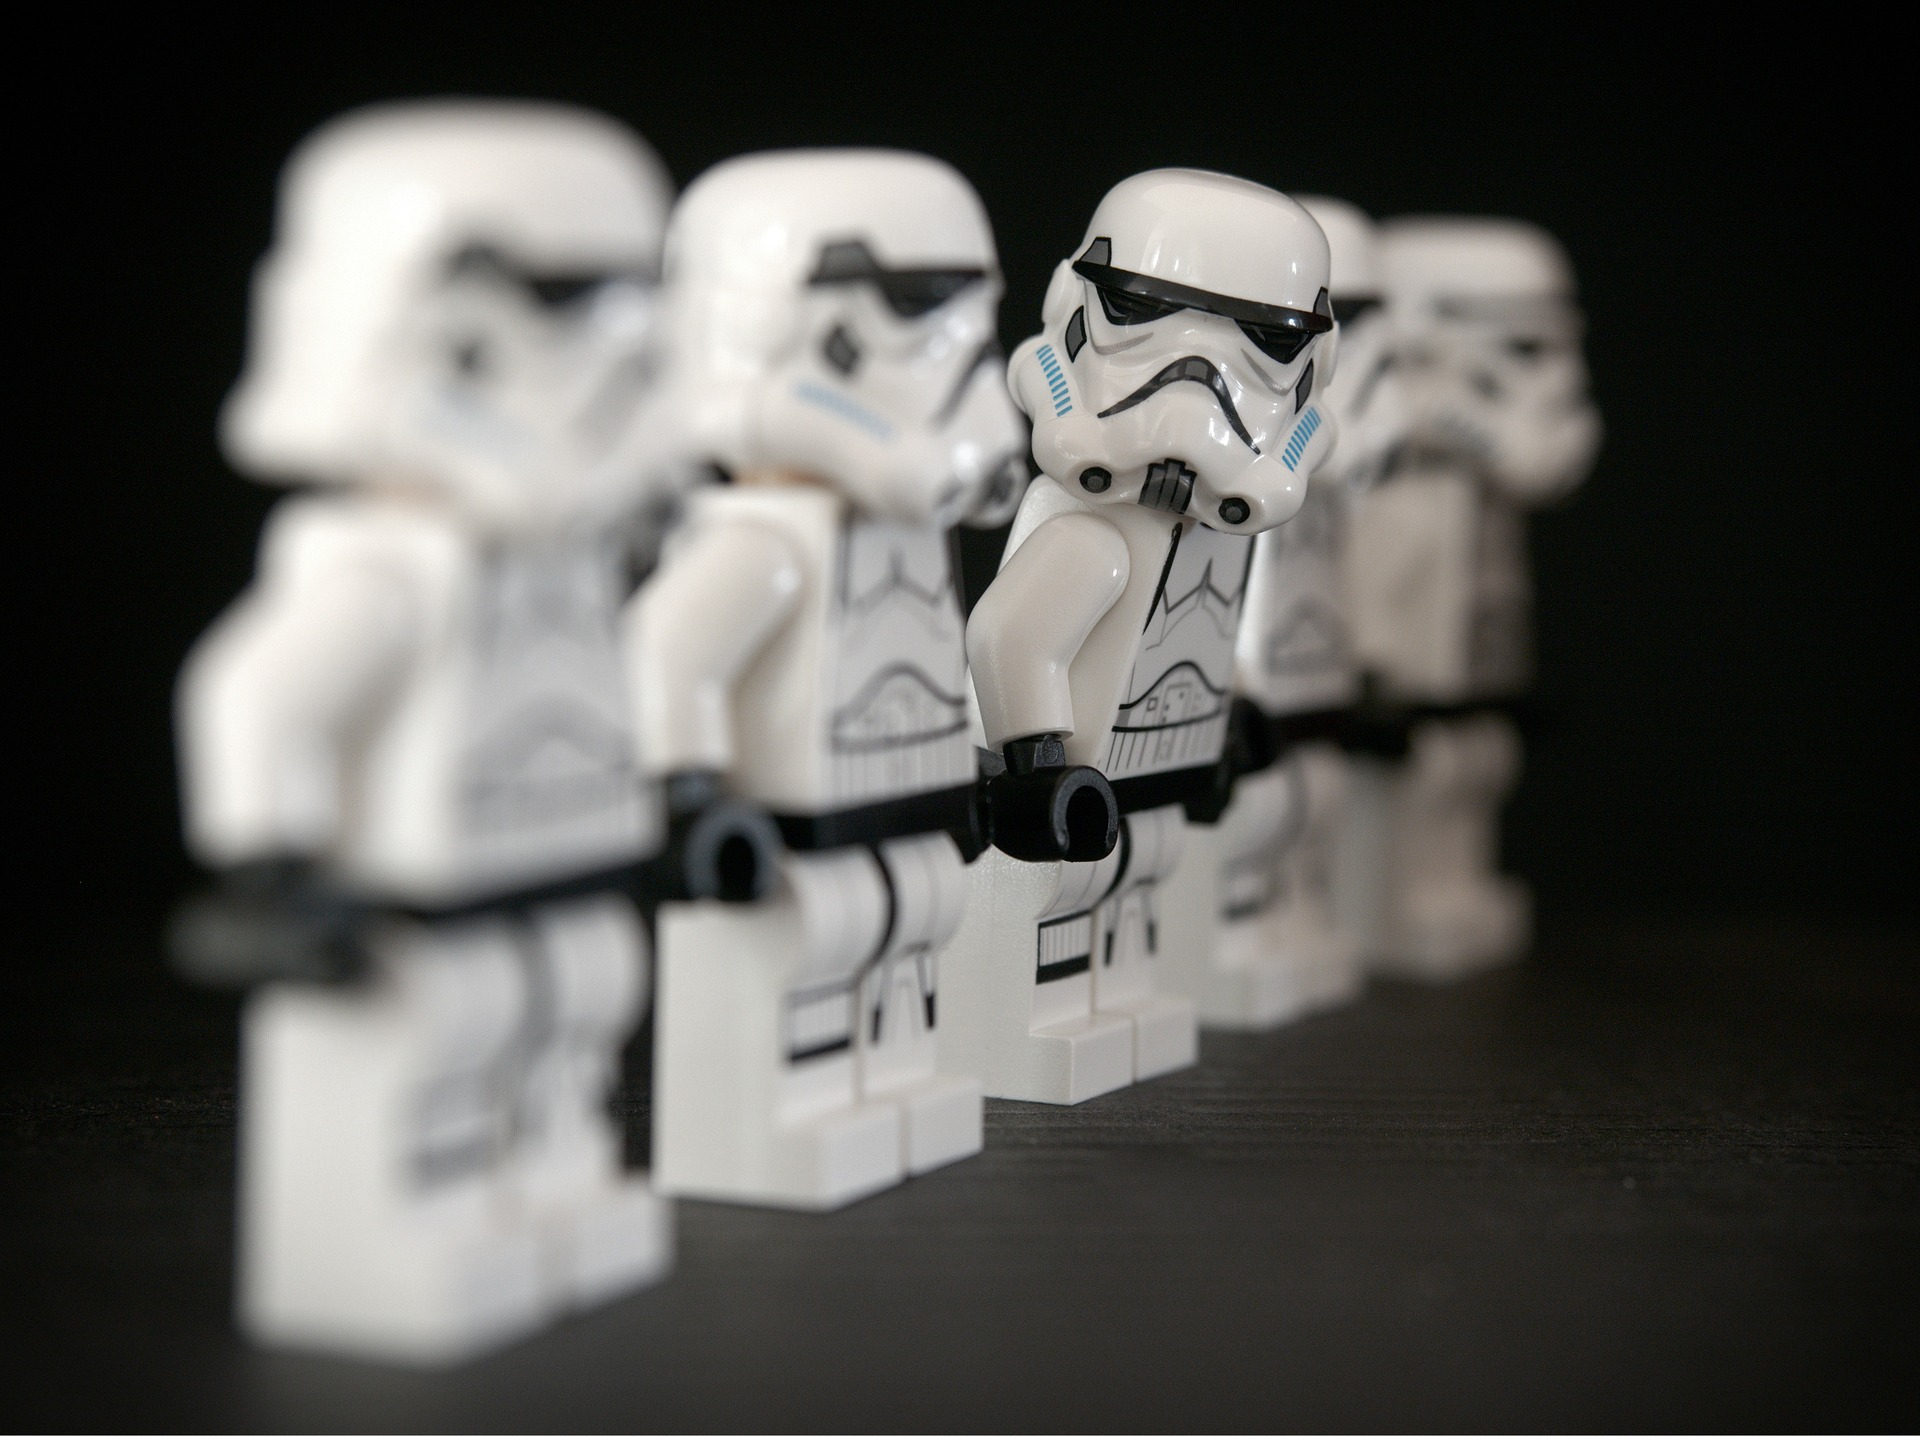
\includegraphics[width=.8\linewidth]{stormtroop.jpg}
\end{center}

\end{frame}
\end{document}